\begin{figure}[b]
    \centering
      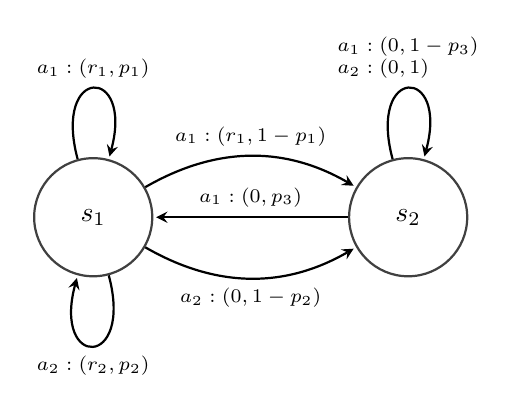
\begin{tikzpicture}[->,>=stealth,shorten >=1pt,auto,node distance=2cm,thick]
        \tikzstyle{state}=[circle,thick,draw=black!75,minimum size=15mm,inner sep=2mm]
        
        \node[state] (A) at (0,0) {$s_1$};
        \node[state] (B) at (4,0) {$s_2$};
        
        \path (A) edge [loop above] node[midway,above, font=\scriptsize] {$a_1:(r_1,p_1)$} 
        (A) edge [loop below] node[midway,below, font=\scriptsize] {$a_2:(r_2,p_2)$} 
        (A)  edge [bend left]  node[midway,above, font=\scriptsize] {$a_1:(r_1,1-p_1)$} (B)
        (B)  edge [out=180, in=360]  node[midway,above, font=\scriptsize] {$a_1:(0,p_3)$} (A)
         (A)  edge [bend right] node[midway,below, font=\scriptsize] {$a_2:(0,1-p_2)$} (B)
    (B) edge [loop above] node[midway,above, font=\scriptsize,align=left] {%
    $a_1:(0,1-p_3)$\\$a_2:(0,1)$} (B);
    \end{tikzpicture}
        \caption{In this MDP (v. \cref{example:non_convexity}),  in each edge it is indicated the action and the corresponding reward and transition probability.}
        \label{fig:example_non_convex_mdp}
\end{figure}